\documentclass[12pt,a4paper]{article}

\usepackage[utf8]{inputenc}
\usepackage[T5]{fontenc}
\usepackage[vietnam]{babel}
\usepackage{geometry}
\usepackage{graphicx}
\usepackage{booktabs}
\usepackage{float}
\usepackage{hyperref}
\usepackage{listings}
\usepackage{xcolor}

\geometry{margin=2.5cm}
\hypersetup{
    colorlinks=true,
    linkcolor=blue,
    urlcolor=blue,
    citecolor=blue
}

\lstdefinestyle{jsonstyle}{
    basicstyle=\ttfamily\small,
    keywordstyle=\color{blue},
    stringstyle=\color{teal},
    numberstyle=\tiny\color{gray},
    breaklines=true,
    frame=single,
    showstringspaces=false
}

\begin{document}

\begin{titlepage}
    \centering
    \vspace*{2cm}
    {\Large \textbf{TRƯỜNG ĐẠI HỌC MỞ TP. HỒ CHÍ MINH}\par}
    \vspace{0.5cm}
    {\large \textbf{BÁO CÁO FINAL PROJECT}\par}
    \vspace{1.5cm}
    {\huge \textbf{Hệ Thống Phân Loại Ý Định Tuyển Sinh}\par}
    \vspace{1.5cm}
    \begin{tabular}{rl}
        \textbf{Môn học:} & \underline{\hspace{8cm}} \\
        \textbf{Giảng viên hướng dẫn:} & \underline{\hspace{7.2cm}} \\
        \textbf{Sinh viên thực hiện:} & \underline{\hspace{7.2cm}} \\
        \textbf{Mã số sinh viên:} & \underline{\hspace{7.2cm}} \\
    \end{tabular}
    \vfill
    {\large TP. Hồ Chí Minh, \today\par}
\end{titlepage}

\tableofcontents
\newpage

\section{Tóm tắt}
Báo cáo trình bày hệ thống phân loại ý định (intent classification) cho bài toán tư vấn tuyển sinh của
Đại học Mở TP. Hồ Chí Minh. Hệ thống sử dụng mô hình \textit{Complement Naive Bayes} kết hợp đặc trưng
TF--IDF, dữ liệu huấn luyện được tăng cường bằng chiến lược loại dấu và mô phỏng lỗi gõ. Kết quả đánh giá
5-fold cross-validation đạt độ chính xác 92.21\% và F1-macro 90.10\%, phù hợp để triển khai dịch vụ suy luận
và giao diện tư vấn trực tuyến.

\section{Giới thiệu}
Nhu cầu tư vấn tuyển sinh ngày càng cao, đòi hỏi hệ thống tự động có thể nhận biết ý định câu hỏi của người dùng
để trả lời nhanh và nhất quán. Dự án \textbf{IntentClassifierOU} xây dựng mô hình phân loại ý định trên
tập dữ liệu câu hỏi tuyển sinh, đồng thời triển khai một API suy luận và giao diện web để tra cứu kết quả.

\section{Mô tả dữ liệu}
Dữ liệu được lưu tại \texttt{data/intents/intents.json}, gồm danh sách \texttt{intents} với các trường:
\texttt{tag}, \texttt{description}, \texttt{examples}, \texttt{response}. Hệ thống hiện có 21 lớp ý định
và tổng cộng 2\,889 mẫu sau tăng cường dữ liệu.

\subsection{Tiền xử lý}
Pipeline tiền xử lý (file \texttt{src/nlp/preprocessor.py}) gồm:
\begin{itemize}
    \item Chuẩn hóa Unicode, chuyển chữ thường, loại ký tự đặc biệt.
    \item Tách từ tiếng Việt bằng \texttt{underthesea} nếu khả dụng.
    \item Loại bỏ stopwords theo miền tuyển sinh.
    \item Tạo thêm biến thể không dấu để tăng độ bao phủ.
\end{itemize}

\subsection{Tăng cường dữ liệu}
Trong quá trình huấn luyện (\texttt{src/classifier/train.py}), dữ liệu được tăng cường bằng:
\begin{itemize}
    \item \textbf{Loại dấu}: sinh thêm câu không dấu.
    \item \textbf{Mô phỏng lỗi gõ}: thay thế cặp ký tự dễ nhầm (ví dụ \texttt{ph} $\rightarrow$ \texttt{f}).
\end{itemize}
Các lớp ngoài phạm vi (\texttt{out\_of\_scope}) được bỏ qua để tránh nhiễu.

\section{Phương pháp}
\subsection{Biểu diễn đặc trưng}
Mỗi câu hỏi được chuyển thành vector TF--IDF với n-gram (1, 2), tối đa 8\,000 đặc trưng, tần suất tối đa 0.95
và áp dụng \textit{sublinear TF}.

\subsection{Mô hình}
Mô hình chính là \textit{Complement Naive Bayes} với hệ số làm trơn $\alpha = 0.1$.
Với vector đặc trưng $\mathbf{x}$, xác suất hậu nghiệm được ước lượng:
\[
P(c \mid \mathbf{x}) \propto P(c)\prod_{i} P(w_i \mid c)^{x_i}
\]
Lớp dự đoán là $\arg\max_{c} P(c \mid \mathbf{x})$.

\section{Huấn luyện và đánh giá}
Huấn luyện được thực hiện theo quy trình:
\begin{enumerate}
    \item Nạp dữ liệu và tăng cường.
    \item Tiền xử lý văn bản.
    \item 5-fold cross-validation để đánh giá tổng quát.
    \item Huấn luyện trên toàn bộ dữ liệu và lưu mô hình tại \texttt{models/intent\_classifier.pkl}.
\end{enumerate}

\subsection{Chỉ số đánh giá}
\begin{table}[H]
    \centering
    \begin{tabular}{l c}
        \toprule
        \textbf{Chỉ số} & \textbf{Giá trị} \\
        \midrule
        Accuracy (CV Prediction) & 0.9221 \\
        Precision (Macro) & 0.9254 \\
        Recall (Macro) & 0.8961 \\
        F1-Score (Macro) & 0.9010 \\
        F1-Macro Mean $\pm$ Std & 0.8988 $\pm$ 0.0246 \\
        Số lớp ý định & 21 \\
        Số mẫu huấn luyện & 2\,889 \\
        \bottomrule
    \end{tabular}
    \caption{Kết quả đánh giá 5-fold cross-validation.}
\end{table}

\subsection{Ma trận nhầm lẫn}
\begin{figure}[H]
    \centering
    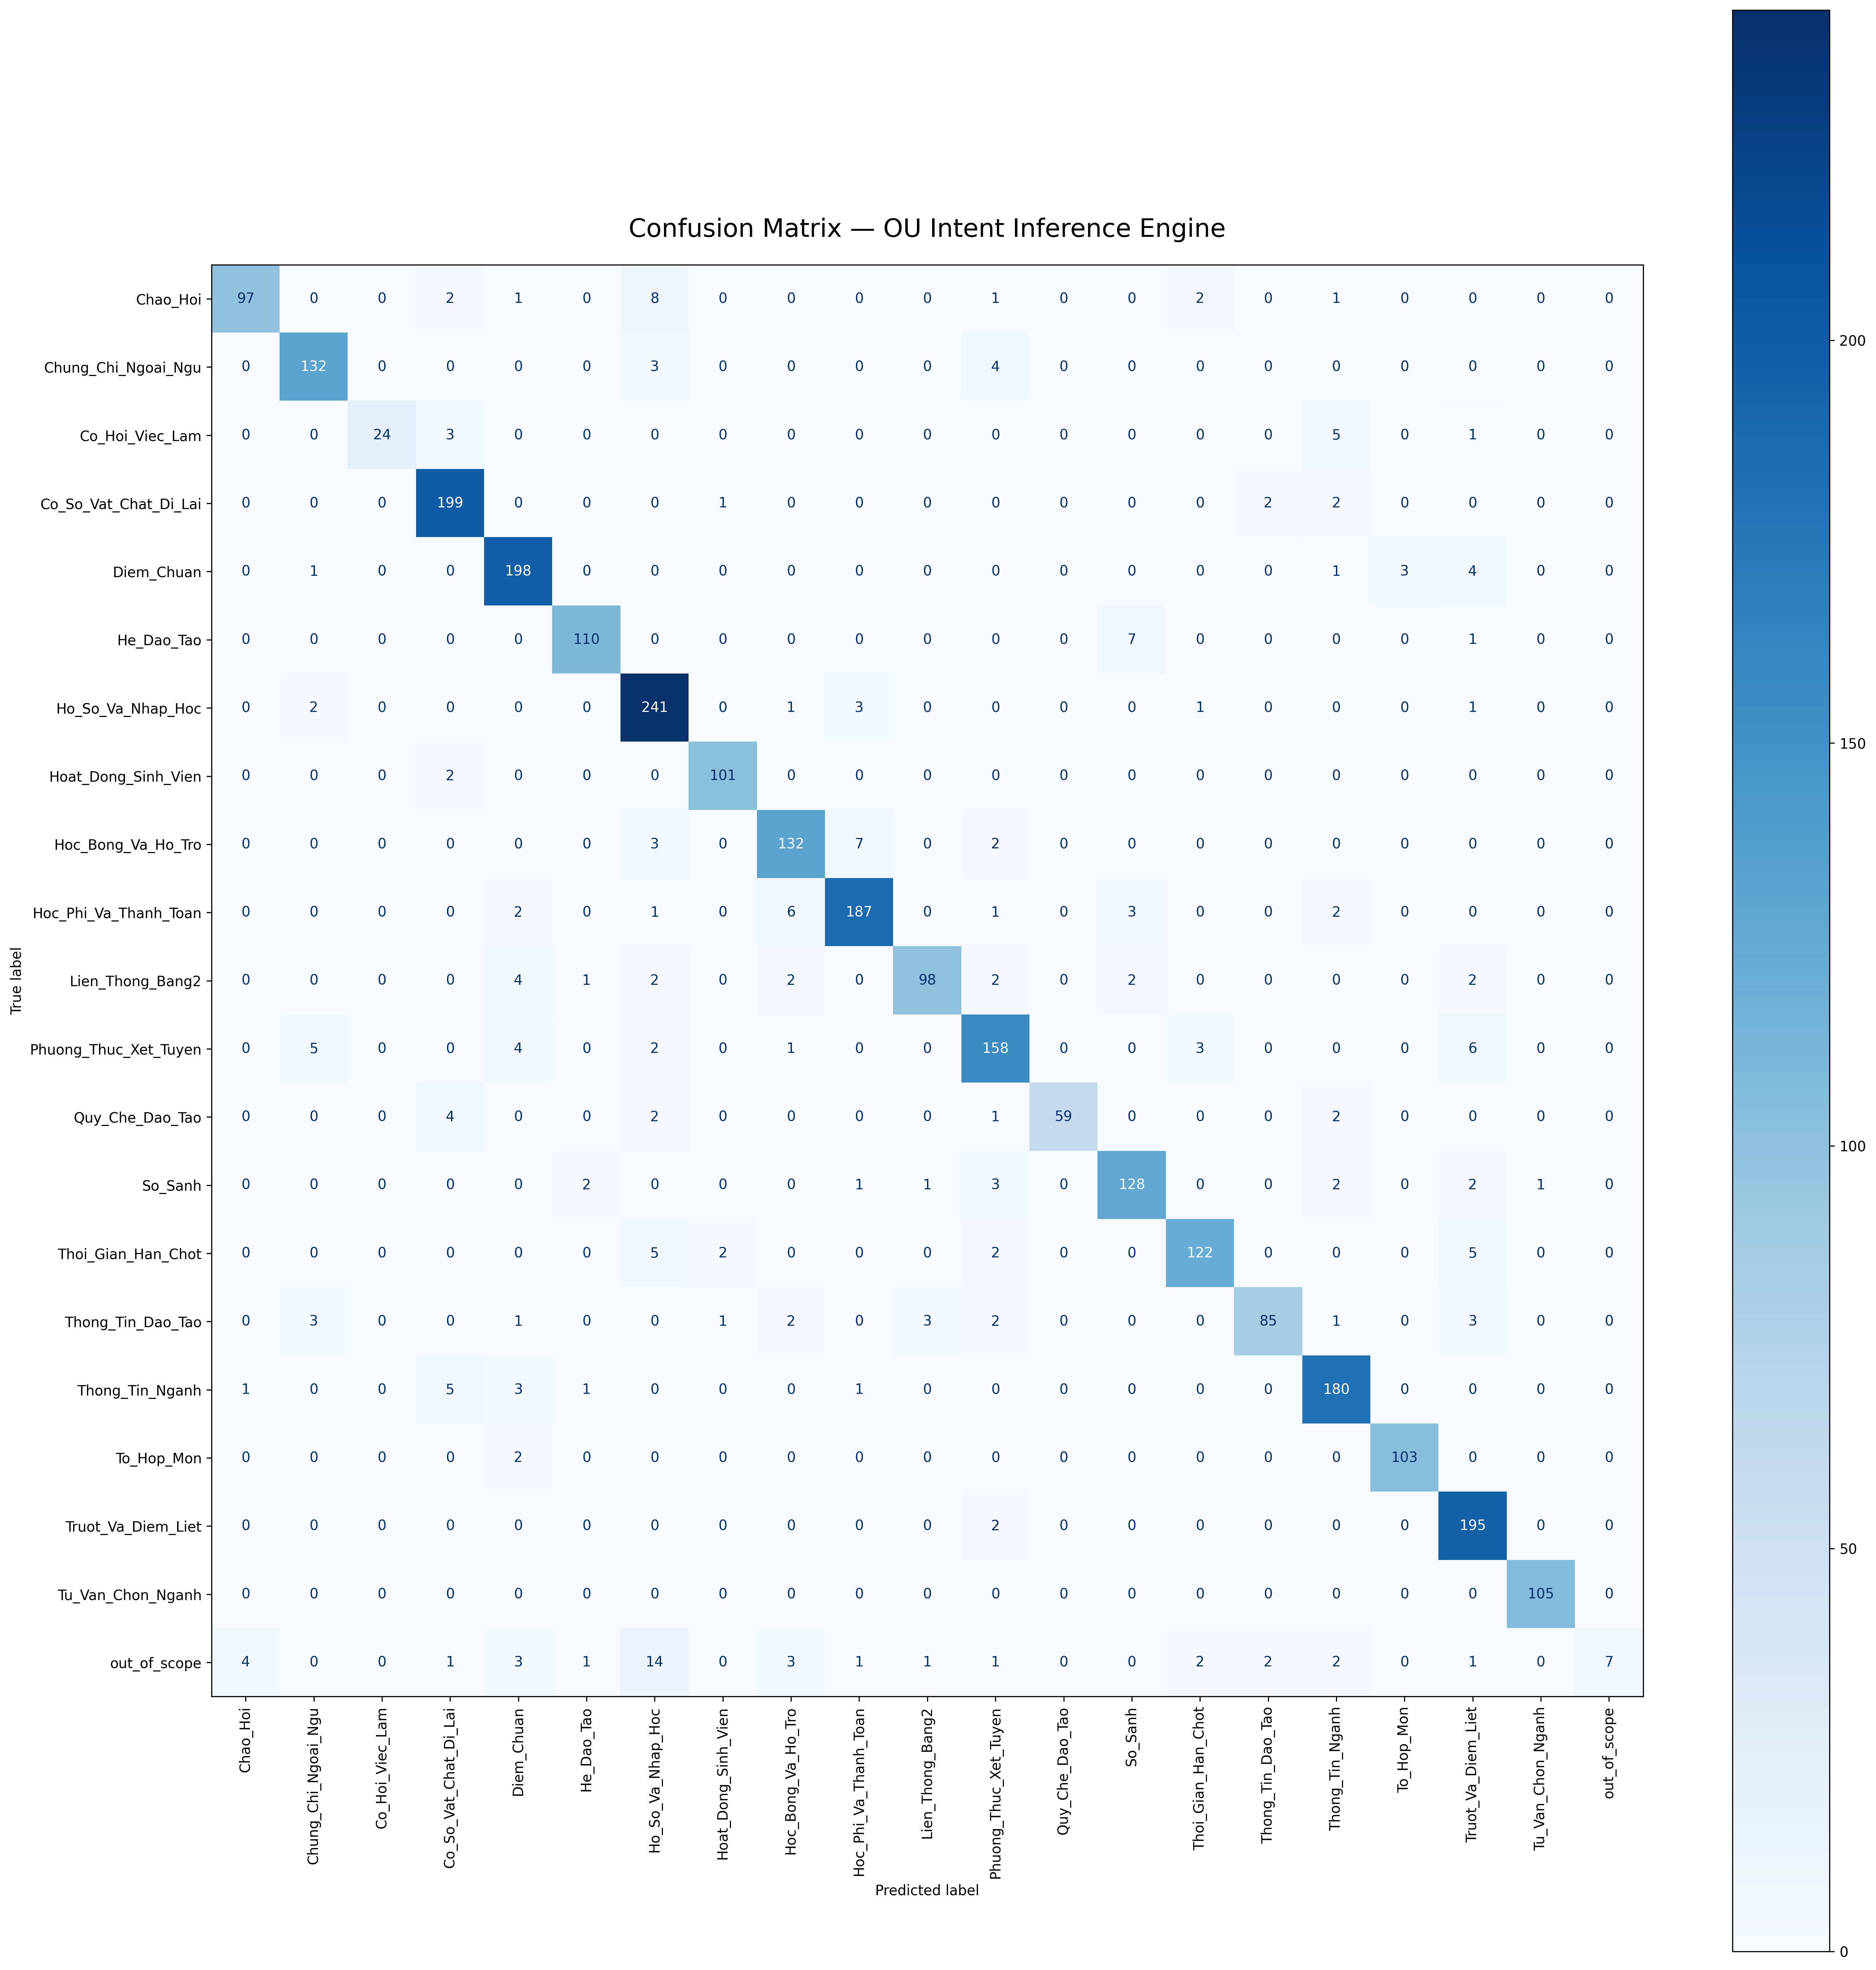
\includegraphics[width=\textwidth]{models/confusion_matrix.png}
    \caption{Ma trận nhầm lẫn theo dự đoán cross-validation.}
\end{figure}

\section{Triển khai hệ thống}
\subsection{Backend}
Backend sử dụng FastAPI (\texttt{backend/backend.py}) với endpoint chính:
\texttt{POST /api/predict}. Dữ liệu vào là JSON gồm trường \texttt{text} và kết quả trả về gồm:
\texttt{intent}, \texttt{confidence}, \texttt{probabilities}, \texttt{top5}. Ví dụ:

\begin{lstlisting}[style=jsonstyle]
POST /api/predict
{
  "text": "Học phí mỗi học kỳ hết bao nhiêu tiền?"
}

Response
{
  "intent": "Hoc_Phi",
  "confidence": 0.93,
  "probabilities": {"Hoc_Phi": 0.93, "...": 0.02},
  "top5": [{"intent": "Hoc_Phi", "prob": 0.93}, ...]
}
\end{lstlisting}

Hệ thống hỗ trợ giới hạn độ dài đầu vào qua biến môi trường \texttt{MAX\_INPUT\_CHARS}
và API key tùy chọn qua header \texttt{X-API-Key}.

\subsection{Frontend}
Frontend xây dựng bằng Streamlit (\texttt{frontend/app.py}), cho phép nhập câu hỏi và hiển thị:
\begin{itemize}
    \item Ý định dự đoán (Maximum A Posteriori).
    \item Độ tin cậy (confidence).
    \item Biểu đồ radar top-6 xác suất lớp.
    \item Thông tin đánh giá mô hình (CV metrics, confusion matrix).
\end{itemize}

\section{Hướng dẫn chạy hệ thống}
\begin{enumerate}
    \item Cài đặt thư viện:
    \begin{lstlisting}[style=jsonstyle]
pip install -r requirements.txt
    \end{lstlisting}
    \item Huấn luyện mô hình:
    \begin{lstlisting}[style=jsonstyle]
python src/classifier/train.py
    \end{lstlisting}
    \item Chạy backend:
    \begin{lstlisting}[style=jsonstyle]
uvicorn backend.backend:app --reload
    \end{lstlisting}
    \item Chạy frontend:
    \begin{lstlisting}[style=jsonstyle]
streamlit run frontend/app.py
    \end{lstlisting}
\end{enumerate}

\section{Kết luận và hướng phát triển}
Hệ thống IntentClassifierOU đạt hiệu quả cao trên dữ liệu tuyển sinh với mô hình nhẹ,
dễ triển khai. Trong tương lai, có thể mở rộng theo các hướng:
\begin{itemize}
    \item Bổ sung dữ liệu và nhãn mới theo từng năm tuyển sinh.
    \item Kết hợp mô hình ngữ cảnh sâu hơn (BERT tiếng Việt) để nâng cao độ chính xác.
    \item Tích hợp cơ chế phản hồi từ người dùng để cải thiện dữ liệu.
\end{itemize}

\begin{thebibliography}{9}
    \bibitem{sklearn} Pedregosa et al., \textit{Scikit-learn: Machine Learning in Python}, JMLR 2011.
    \bibitem{underthesea} Underthesea NLP Toolkit, \url{https://github.com/undertheseanlp/underthesea}.
\end{thebibliography}

\end{document}
